\begin{minipage}[t]{0.15\textwidth}
	\centering
	\vspace{0pt}
	
	\caption*{(1)}
	
	\tikzsetnextfilename{huffman-tree-simple-shapes-1}
	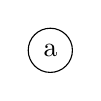
\begin{tikzpicture}[edge from parent/.style = { draw, -latex }]
	\node [draw, circle] { a };
	\end{tikzpicture}
\end{minipage}
\begin{minipage}[t]{0.25\textwidth}
	\centering
	\vspace{0pt}
	
	\caption*{(2)}
	
	\tikzsetnextfilename{huffman-tree-simple-shapes-2}
	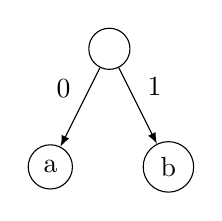
\begin{tikzpicture}[edge from parent/.style = { draw, -latex }]
	\node [draw, circle] { \phantom{-} }
	child {
		node [draw, circle] { a }
		edge from parent node [above left] { 0 }
	}
	child {
		node [draw, circle] { b }
		edge from parent node [above right] { 1 }
	};
	\end{tikzpicture}
\end{minipage}
\begin{minipage}[t]{0.29\textwidth}
	\centering
	\vspace{0pt}
	
	\caption*{(3)}
	
	\tikzsetnextfilename{huffman-tree-simple-shapes-3}
	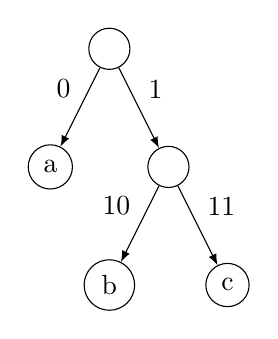
\begin{tikzpicture}[edge from parent/.style = { draw, -latex }]
	\node [draw, circle] { \phantom{-} }
	child {
		node [draw, circle] { a }
		edge from parent node [above left] { 0 }
	}
	child {
		node [draw, circle] { \phantom{-} }
		child {
			node [draw, circle] { b }
			edge from parent node [above left] { 10 }
		}
		child {
			node [draw, circle] { c }
			edge from parent node [above right] { 11 }
		}
		edge from parent node [above right] { 1 }
	};
	\end{tikzpicture}
\end{minipage}

\bigskip
\bigskip

\begin{minipage}[t]{0.38\textwidth}
	\centering
	\vspace{0pt}
	
	\caption*{(4)}
	
	\tikzsetnextfilename{huffman-tree-simple-shapes-4}
	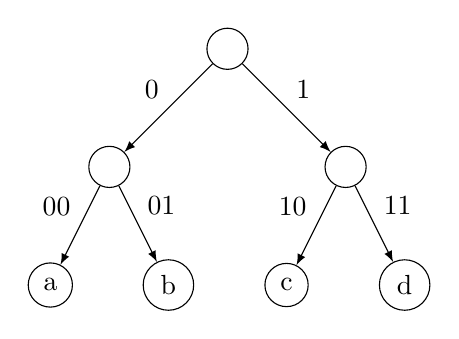
\begin{tikzpicture}[
		edge from parent/.style = { draw, -latex },
		level 1/.style = { sibling distance = 2\tikzsiblingdistance },
		level 2/.style = { sibling distance = 0.5\tikzsiblingdistance }
	]
	\node [draw, circle] { \phantom{-} }
	child {
		node [draw, circle] { \phantom{-} }
		child {
			node [draw, circle] { a }
			edge from parent node [above left] { 00 }
		}
		child {
			node [draw, circle] { b }
			edge from parent node [above right] { 01 }
		}
		edge from parent node [above left] { 0 }
	}
	child {
		node [draw, circle] { \phantom{-} }
		child {
			node [draw, circle] { c }
			edge from parent node [above left] { 10 }
		}
		child {
			node [draw, circle] { d }
			edge from parent node [above right] { 11 }
		}
		edge from parent node [above right] { 1 }
	};
	\end{tikzpicture}
\end{minipage}
\begin{minipage}[t]{0.36\textwidth}
	\centering
	\vspace{0pt}
	
	\caption*{(5)}
	
	\tikzsetnextfilename{huffman-tree-simple-shapes-5}
	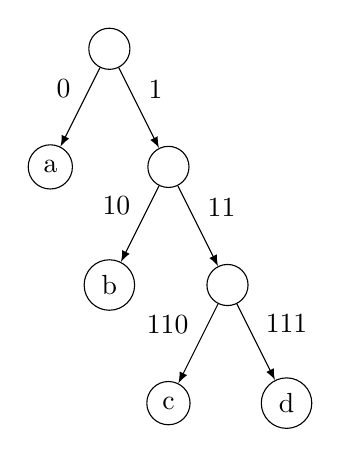
\begin{tikzpicture}[edge from parent/.style = { draw, -latex }]
	\node [draw, circle] { \phantom{-} }
	child {
		node [draw, circle] { a }
		edge from parent node [above left] { 0 }
	}
	child {
		node [draw, circle] { \phantom{-} }
		child {
			node [draw, circle] { b }
			edge from parent node [above left] { 10 }
		}
		child {
			node [draw, circle] { \phantom{-} }
			child {
				node [draw, circle] { c }
				edge from parent node [above left] { 110 }
			}
			child {
				node [draw, circle] { d }
				edge from parent node [above right] { 111 }
			}
			edge from parent node [above right] { 11 }
		}
		edge from parent node [above right] { 1 }
	};
	\end{tikzpicture}
\end{minipage}